\begin{figure}[H]
    \centering
    \begin{minipage}{0.33\textwidth}
        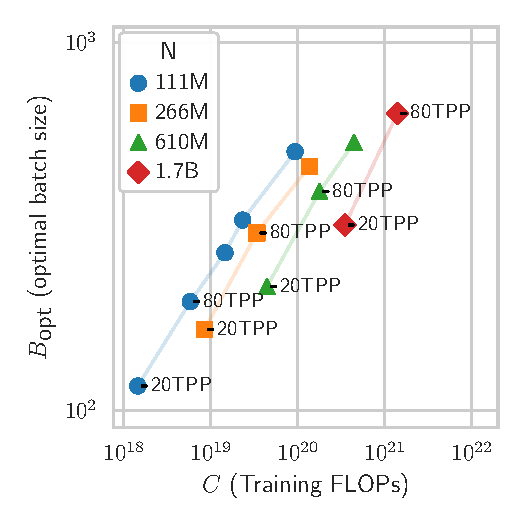
\includegraphics[trim={0.3cm 0.4cm 0.3cm 0.3cm}, clip, width=\linewidth]{pdffigs/bopt_scaling_law.mydata.C.pdf}
    \end{minipage}\hfill
    \begin{minipage}{0.33\textwidth}
        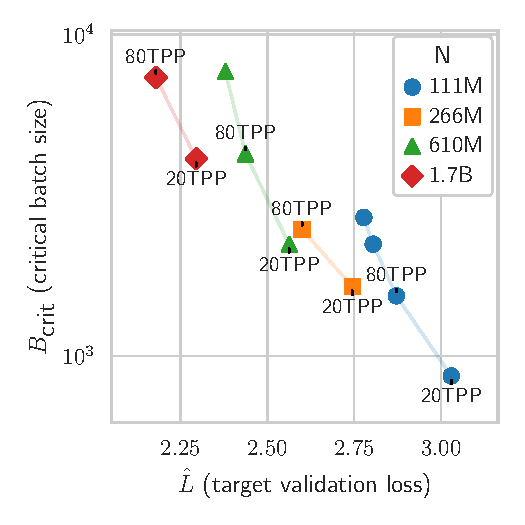
\includegraphics[trim={0.3cm 0.4cm 0.3cm 0.3cm}, clip, width=\linewidth]{pdffigs/loss_data.241005.cbs_scaling.target_loss.pdf}
    \end{minipage}\hfill
    \begin{minipage}{0.33\textwidth}
        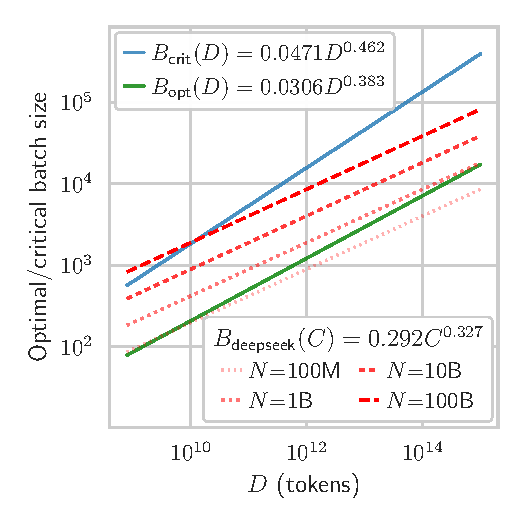
\includegraphics[trim={0.3cm 0.4cm 0.3cm 0.3cm}, clip, width=\linewidth]{pdffigs/b_all_scaling.pdf}
    \end{minipage}
    \caption{Prior work suggests $\bopt$ scales in $C$ ($\leftfig$)
      and $\bcrit$ in loss ($\middlefig$), but \emph{this only holds
      at a fixed $N$/TPP} (same data as \cref{fig:hook}
      $\middlefig$/$\rightfig$); \cref{fig:hook} shows scaling in $D$
      is the fundamental relationship.
      %
      Plotting $\bdeepseek(C)$ law from~\citet{bi2024deepseek}
      ($\rightfig$), but over $D$ (using $C \approx 6ND$ to obtain $C$
      for the spurious dependence on $N$), we see
      \citet{bi2024deepseek} used generally efficient $B$ values
      (i.e., within the $\bopt < B < \bcrit$ regime) despite fitting $C$
      rather than $D$ ($\bopt$ and $\bcrit$ lines from
      \cref{fig:hook}).\label{fig:related}}
\end{figure}
